\chapter{The LTLCreator prototype}
\label{chap:theltlcreatorprototype}

As stated in chapter~\ref{chap:goals}, appropriate support by a graphical editor is important for the usefulness of the developed visual language. We therefore designed and implemented a prototype of such an editor which contains the visual language as well as the proposed constraint generation heuristics. The implementation is a java swing component and has a simple API definition, making it easy to integrate the LTLCreator tool into other java applications.

First of all some details about the implementation of the visual language are given in section~\ref{sec:prototype:operatorconstraints}, directly followed by an explanation about the realization of the automated constraint generation functionality in section~\ref{sec:prototype:automatedconstraintgeneration}.
The assembly of all the previous features in one tool is described in section~\ref{sec:coalescence}. However, the tool's functionality shall also be available in Robostudio in order to provide safety mechanisms for the healthcare service robots and to be a prototype for evaluation. Section~\ref{sec:integrationintorobostudio} gives a main idea how an integration into Robostudio ought to be. 



\section{Operator constraints}
\label{sec:prototype:operatorconstraints}

Each of the different operator types, i.e. IfThenOperator, AndOperator, OrOperator, NotOperator, NextOperator, FutureOperator, AlwaysOperator, UntilOperator and StateOperator, has got its own representing class. All of them inherit from one abstract class AbstractOperator which provides the basic functionality beeing used by all operators. The AbstractOperator class is shown in figure~\ref{fig:abstractoperator} and its methods are described as follows:

\begin{description}
	\item[getLTL():] This function returns the LTL formula of an operator and all its children recursively. Applied to the most outer operator it returns the complete formula for the constraint. This function is abstract and implemented by each operator type separately.
	\item[getColor():] Each operator type has got is own significant color which can be retrieved over the abstract function getColor().
	\item[createNewInstance():] In order to provide operator creation over a tool bar, this function instantiates a new operator object dependet on the implementation.
	\item[setMouseOver(boolean):] Mouse over actions cause the underlying operator to be highlighted. This function makes all operators except the hovered one appearing bleeched out.
	\item[paintOperator(Graphics, ...):] Each operator class has to implement the abstract function paintOperator(). It manages all color and shape painting for the respective operator. Additional parameters such as recursive painting including children can be spezified.
	\item[contains(int, int):] Given two coordinates x and y, it can be determined wheter the herewith defined point lays within an operator.
	\item[isSimilar(AbstractOperator):] Two operators can be compared for semantic equality. That means same operators with same children. This functionality is important for avoiding duplicate constraints during constraint generation.
	\item[addChangeListener(OperatorChangeListener):] Whenever there is a change to the operator or one of its children, an operator change listener gets notified about it. The hierarchical architecture of AbstractOperators propagates all change events to the root operator. The function addChangeListener() allows registering for such change notifications.
	\item[removeChangeListener(OperatorChangeListener):] According to addChangeListener this function allows deregistration again.
\end{description}

\begin{figure}[htbp]
  \centering
  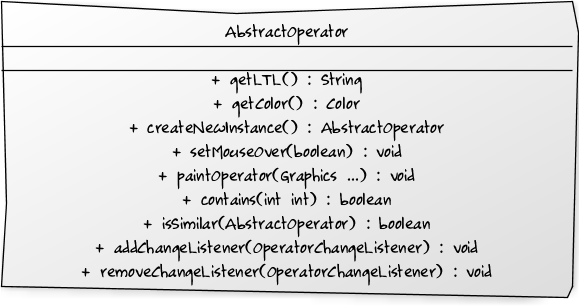
\includegraphics[width=0.6\linewidth]{AbstractOperator} 
  \caption{AbstractOperator class definition.}
  \label{fig:abstractoperator}
\end{figure}

Whereas StateOperators have got no operator children and are leafs in the syntax tree of LTL formulas, all other operator types are either unary or binary operators with respective one or two possible children. 
The graphical representation of both unary and binary operators thus needs to have place holders and docking stations for sub operators. These are realized by buckets which display a small ``drop here'' label and allow operator adding or removing by mouse drops. For this a class Bucket is defined with get and set methods for defining a sub operator.
Figure~\ref{fig:klassendiagramm_operators} depicts the relationship between AbstractOperator, Bucket and operator implementations.

\begin{figure}[htbp]
  \centering
  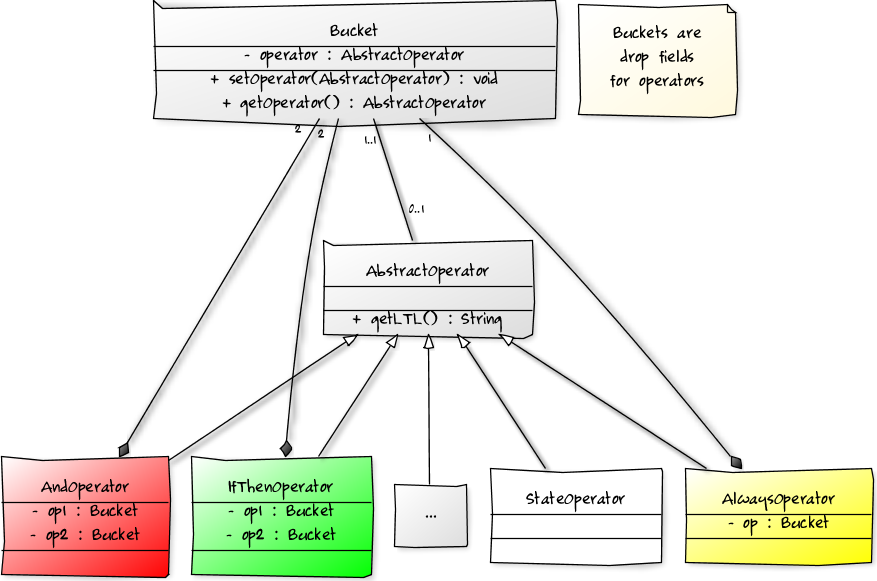
\includegraphics[width=\linewidth]{klassendiagramm_operators} 
  \caption{Class diagram of operator structure.}
  \label{fig:klassendiagramm_operators}
\end{figure}

Once operators are composed in a way that no empty buckets are left over, we retrieve a complete constraint such as the one shown in figure~\ref{fig:operator_tree}. This diagram illustrates the correlation of nested operators and buckets.

\begin{figure}[htbp]
  \centering
  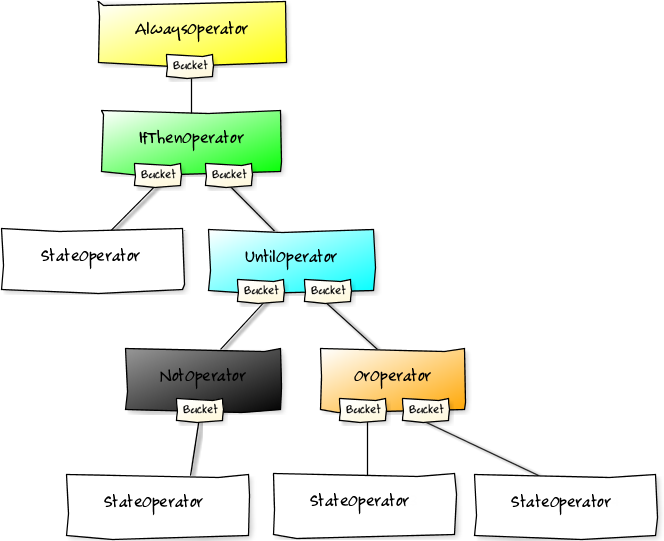
\includegraphics[width=\linewidth]{operator_tree} 
  \caption{Instantiation of a constraint with several operators.}
  \label{fig:operator_tree}
\end{figure}

All graphical components such as buckets and operators are implemented as java swing JComponent. Thereby a lot of functionality for the visual configuration is already available such as the complex layout and repaint concept and the container functionality which is used for unary and binary operators as well as buckets.

%PAINT

For lightweight components swing allows the implementation of a paint() method which is responsible for rendering the component. This is used for giving every operator its special look. We hereby made use of swing's Graphics2D functionality what gives a great support in painting rounded shapes and color gradients. An operator is displayed as a rounded rectangle with dents around sub operators and has got a flowing backgound, borders and labels in an operator type specific color. For the significant shape multiple rounded rectangles with and without border are arranged in a way that the result appears to be one peace. Figure~\ref{fig:paintprocess} demonstrates how the process of painting is: For painting the if operator first of all a blank rectangle with border is drawn, directly followed by two filled rectangles with border which are placed where later the two child operators shall be. In the third step the same rectangle as from step one just this time without border is painted on top. This makes all crossing borders disappear. Only labels and buckets have to be added yet and a complete IfThenOperator emerges.

\begin{figure}[htbp]
  \centering
  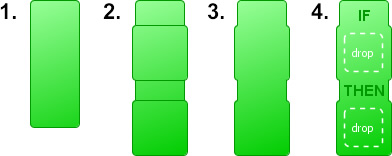
\includegraphics[scale=0.65]{paintprocess} 
  \caption{Steps of painting an operator.}
  \label{fig:paintprocess}
\end{figure}

%Um die paint-Logik muss sich nicht gek�mmert werden, lediglich die paint mehtode muss implementiert werden, die dem jeweiligen Operator sein spezielles Aussehen verleiht. Dabei wurde auf die Funktionen des Graphics2D zur�ckgegriffen, was die Erstellung von runden Formen (shapes) und Farbverl�ufen (stroke?) erm�glicht. Jeder Operatortyp hat eine spezifische Farbe, die f�r den Farbverlauf im Hintergrund, f�r den Border und als Textfarbe verwendet wird. Die shapes der Operatoren wurden so umgesetzt, dass sie sich um die enthaltenen Operatoren schlingen (schmiegen). Hierf�r wurden auschlie�lich leere und gef�llte abgerundete Rechtecke gezeichnet, die in der richtigen Reihenfolge �bereinandergelegt die gew�nschte Endform f�r den Operator ergibt. grafisches beispiel?

%LAYOUT

Swing also provides a mechanism for layouting components, that means depending on child components the aspired sizes and positions of components can be retrieved. As known from figure~\ref{fig:operators} in section~\ref{sec:operatorconstraints} constraints have particular meanings for the two dimensions: a vertical read direction and the horizontal direction for varation in time. This fact forms a special requirement for the layouting of operators.
Whereas the operator's positioning and resizing along the logical direction is only dependend on the sizes of sub operators, the arrangement within the time axis turns out to be more difficult. Here sub operators can't just be aligned centered as it is the case vertically. To face the determination of horizontal positioning, every operator gets time reference lines as depicted in figure~\ref{fig:referencelines}. Logical operators, i.e. IfThenOperator, AndOperator, OrOperator, NotOperator and StateOperator, have one reference line, time relevant operators, i.e. NextOperator, FutureOperator, AlwaysOperator and UntilOperator, have two such reference lines.

\begin{figure}[htbp]
  \centering
  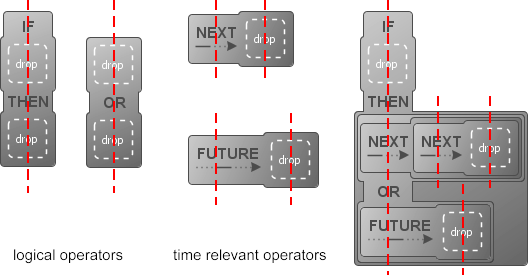
\includegraphics[scale=0.65]{referencelines} 
  \caption{Time reference lines and their adjustment.}
  \label{fig:referencelines}
\end{figure}

%�ber den eingebauten Layoutmanager-Mechanismus kann die Anordnung der Operatoren zueinander festgelegt werden. Wie aus section xy bekannt, gibt es eine logische wie auch eine zeitliche Achse bei constraints. Demnach muss die verticale wie auch horizontale positionierung der operatoren bestimmt werden. jeder operator besitzt eine logische Mittellinie, die wird zur mittellinie des �bergeordneten Buckets ausgerichtet.

%DRAG&DROP

The inbuilt mouse support of swing was used for identifying operators laying under the current mouse position. On the one hand this is important for mouse sensitive highlighting of particular constraint parts, on the other hand this way it can be determined where operators have to be added after drag and drop. So far the predefined swing drag and drop has not been used but a simple drag and drop handler has been implemented instead. Once a JComponent is registered to the class DndHandler, it automatically manages any drag and drop actions with JComponents which implement either the Draggable or DropTarget interface. The former is implemented by all operators, the latter by buckets and the dashboard.
%Figure~\ref{fig:dndclassstructure} gives a short class overview.
Furthermore there is a class DraggableProvider which displays a kind of button in the tool bar and lets the user create new Draggables; in our case new operators get instantiated.

%das vorgefertigte Mouse-Handling wurde verwendet, um die jeweilige operator oder bucket componente an der aktuellen mausposition zu bestimmen. Die ist zum einen wichtig bei dar�berfahrender maus um Teile des constraints hervorzuheben, zum anderen wird damit beim draggen auch bestimmt, welcher operator verschoben werden soll oder an welche stelle einer abgelegt werden soll.

\begin{figure}[htbp]
  \centering
  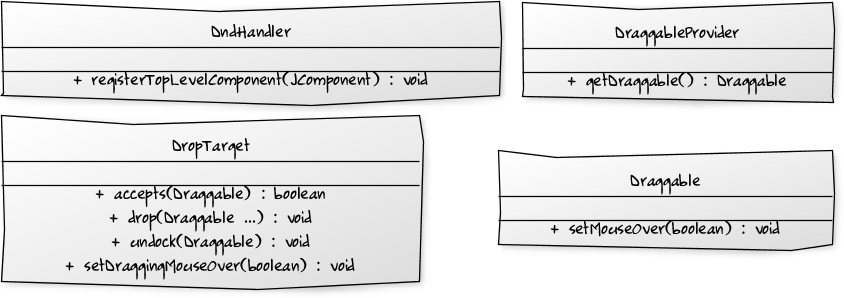
\includegraphics[width=\linewidth]{dndclassstructure} 
  \caption{Class definition of drag and drop functionality.}
  \label{fig:dndclassstructure}
\end{figure}


%operator werden im dashboard, einem weiteren container, zusammengeklickt und angezeigt. Das Dashboard hat dabei eine �hnliche Funktionsweise wie ein Bucket. die operatoren k�nnen dabei vom operatorprovider bezogen werden: Implementierungsdetails? trash...






\section{Automated constraint generation}
\label{sec:prototype:automatedconstraintgeneration}

% (on huge state machines) (brute force algorithm)
 
%Da der subgraph-finde-algorithmus als brute force algorithmus implementiert wurde, der saemtliche sub graphs durch Abwandern s�mtlicher Pfade der zugrundeliegenden state machine herauszufinden versucht, kann bei grossen programmen (ab ca. 1000 Zustaenden und sehr vielen Verzweigungen) der findeprozess teils sehr lange (mehrere Minuten) dauern. Um den warteprozess ertraelicher zu machen wird w�hrend der findung ein dialog mit dem aktuellen fortschritt und einem abbrechen button angezeigt.







\section{Coalescence}
\label{sec:coalescence}

Both features the visual language presented in section~\ref{sec:operatorconstraints} and the automated constraint generation in chapter~\ref{chap:automatedconstraintgeneration} have to be assembled in one tool, the LTLCreator. It shall provide a dashboard with the possibility to manage several constraints, such as a tab panel, and displays for indicating validation results. Besides a button is needed for triggering constraint generation.


TODO: beschreiben dass vl im tab eingebunden wurde, die constraintgenerierung unter den zauberstab.


Figure~\ref{fig:editor} shows a snapshot of the editor's environment: All functionality needed for constraint editing is provided in the tool bar on the right. It contains draggable elements for creating all operator and proposition types as well as a trashcan for deleting. Constraints can be composed in the dashboard in the center of the editor by drag\&drop which holds and displays the operator constraints. The tab functionality on the left allows multiple constraints to be managed. Each tab shows a small thumbnail of the constraint and a symbol indicating its validity; a warning shield for ``incomplete'', a green shield for ``valid'', a red cross for ``invalid'' or an animated ring for ``validation in progress.''. The magic wand button within the tab pane brings the constraint generation functionality into the editor and triggers the constraint finding process.

\begin{figure}[htbp]
  \centering
  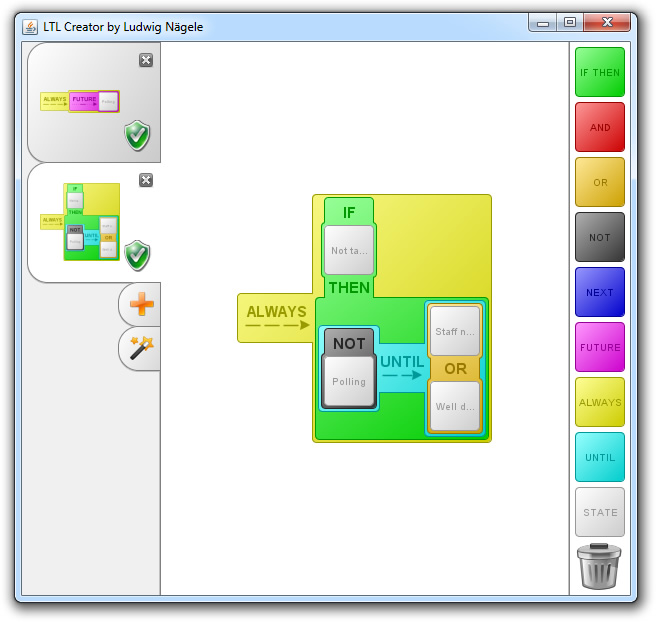
\includegraphics[width=\linewidth]{editor} 
  \caption{Snapshot of the visual editor.}
  \label{fig:editor}
\end{figure}










\subsection{Model checker}

NuSMV
warum den? Davor verwendete erwaehnen?

a CTL model checker has been written in java, but...

Furthermore a particular model checker can be specified for constraint validation. As a default, the symbolic model checker NuSMV~\cite{springerlink:10.1007/s100090050046,NuSMV2} is used.

wie genau wird das getriggert (rekursiver listener an operatoren)

ConstraintValidator
ValidatorThread

(im hintergrund, mit warteschlange. dabei sollen aber wenn ein contsraint frequently ge�ndert wird, alte validationsauftr�ge des gleichen constraints aus der warteschlange entfernt werden.
Callback mit result.



%\subsection{Integratability}
\subsection{Ease of integration}

LTLCreator should be available for other state machine based programming environments for integration what is ensured by its implementation as a java swing component and a clear API enabling the tool for a wide range of use.

Figure~\ref{fig:coalescence} points out how interaction between LTLCreator and programming environments where it is integrated in can be.
LTLCreator consists of a dashboard where constraints can be edited visually and an graphical output of validation results. The constraint generator as well as the validator are non UI parts of LTLCreator.
The programming environment provides the state machine model and notifies the LTLCreator component about all changes made to the program. This will automatically revalidate all existing constraints and always provide the up-to-date model for constraint generation.
For load and save functionality, all existing constraints can be received and new ones can be added to the LTLCreator component programmatically.

\begin{figure}[htbp]
  \centering
  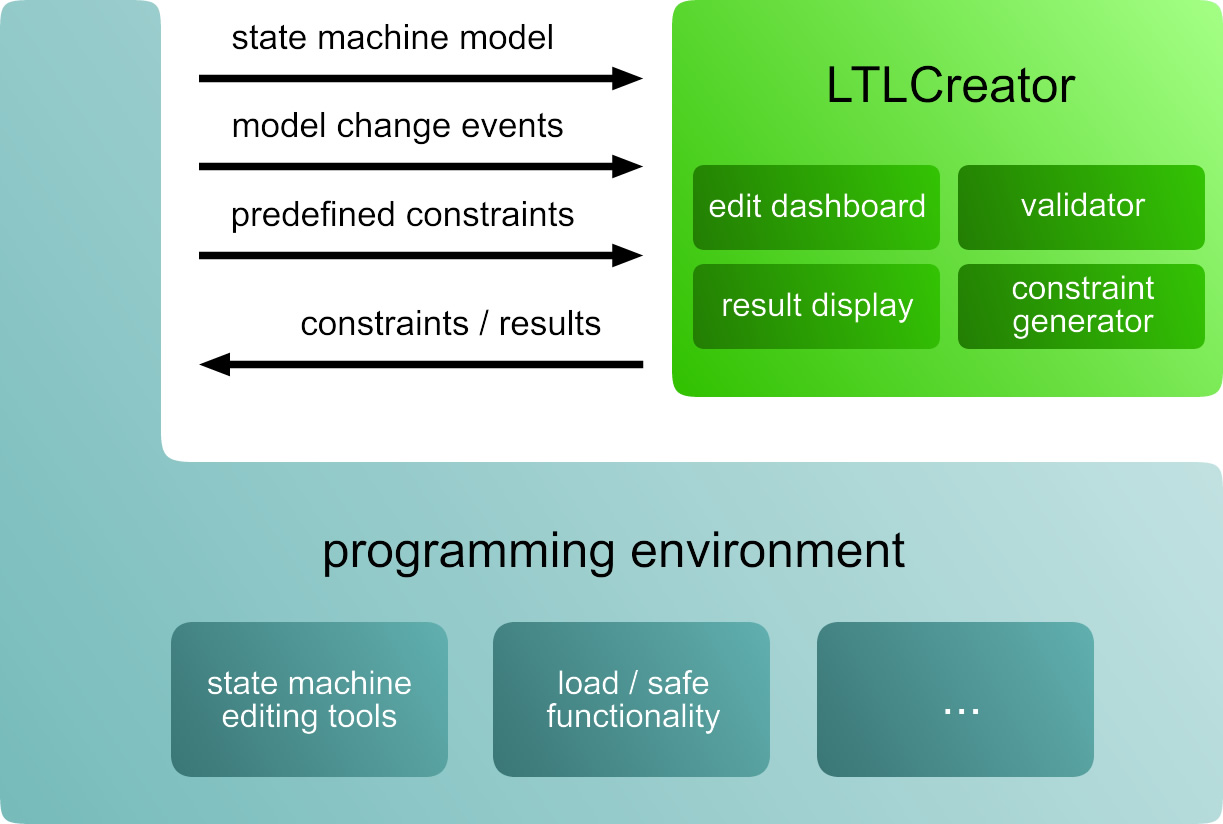
\includegraphics[width=0.7\linewidth]{coalescence}
  \caption{Interaction between LTLCreator and programming environment.}
  \label{fig:coalescence}
\end{figure}







\section{Integration into Robostudio}
\label{sec:integrationintorobostudio}

kurz erl�utern, warum das gemaacht werden soll

Robostudio uses NetBeans as a platform, and all tools and features are organized in windows. Thus also LTLCreator has to be put into a window and added to the Robostudio platform. Since the defining of safety constraints is an important part not only after but also during the process of developing service robot behavior, the LTLCreator window as a vital tool shall be placed in the center of the platform where currently also the UI Component Layout Editor Window is. As already proposed in the previous section, all changes to the state machine program made within robostudio must of course cause the LTLCreator window to revalidate all existing constraints.




allein benutzbar, oder ueber robostudio, automatische synchronisierung mit model

%Since Robostudio uses NetBeans as a platform, the LTLCreator has to be integrated as a NetBeans component. Die Datenanbindung zum Austausch des modells (Zustandsmaschine) und der Constraints erfolgt hierbei durch �ffentliche




\subsection{Problems}

(auto-revalidation, model-errors, ...?)
nicht EINE zentrale stelle f�r model�nderungen => zer\-pfl�ck\-te programmierung, wenn man alle �nderungen haben will




\subsection{Solutions}

(pre-checker)

statische analyse